%% This is an example first chapter.  You should put chapter/appendix that you
%% write into a separate file, and add a line \include{yourfilename} to
%% main.tex, where `yourfilename.tex' is the name of the chapter/appendix file.
%% You can process specific files by typing their names in at the 
%% \files=
%% prompt when you run the file main.tex through LaTeX.
\chapter{Experiments}
\label{chap:experiments}

% % remove all spaces between columns in tables
% \setlength{\tabcolsep}{0.3pt}
% % remove all spaces below captions
% \setlength{\belowcaptionskip}{-5pt}

In this chapter, we first introduce our synthetic dataset. This dataset contains IMU measurements and corresponding visual frames, it also provides the ground truth IMU-camera pose to be used in evaluation stage. We then perform several experiments to show that our visual-inertial odometry has good accuracy and low computational cost with different experimental settings.

\section{Synthetic Dataset}
\label{sec:sync_data}

\begin{table}[t]
\centering
\begin{tabular}{|c || P{2.5cm} | P{2.5cm} | P{6.5cm}|} 
\hline
 Name & Duration $\left[ s \right]$ & Distance $\left[ m \right]$ & Description \\
 \hline
 001 & 30.0 & 165.97 & Pure movement without rotation \\ 
 002 & 30.0 & 0.0 & Pure rotation without translation \\ 
 003 & 30.0 & 118.99 & Random straight trajectory \\ 
 004 & 120.0 & 257.71 & Random circle trajectory \\ 
 \hline
\end{tabular}
     \caption{Trajectories we create for experiments, the datasets are named after the corresponding trajectories. Note that \textbf{001} and \textbf{002} are ideal trajectories in order to evaluate the correctness and performance of ESKF IMU integration. The trajectory \textbf{003} and \textbf{004} try to simulate different types of real micro helicopter trajectories.}
    \label{table:tb1}
\end{table}

%\begin{figure}
%\centering
%	\begin{subfloat}[Trajectory 003]{
%		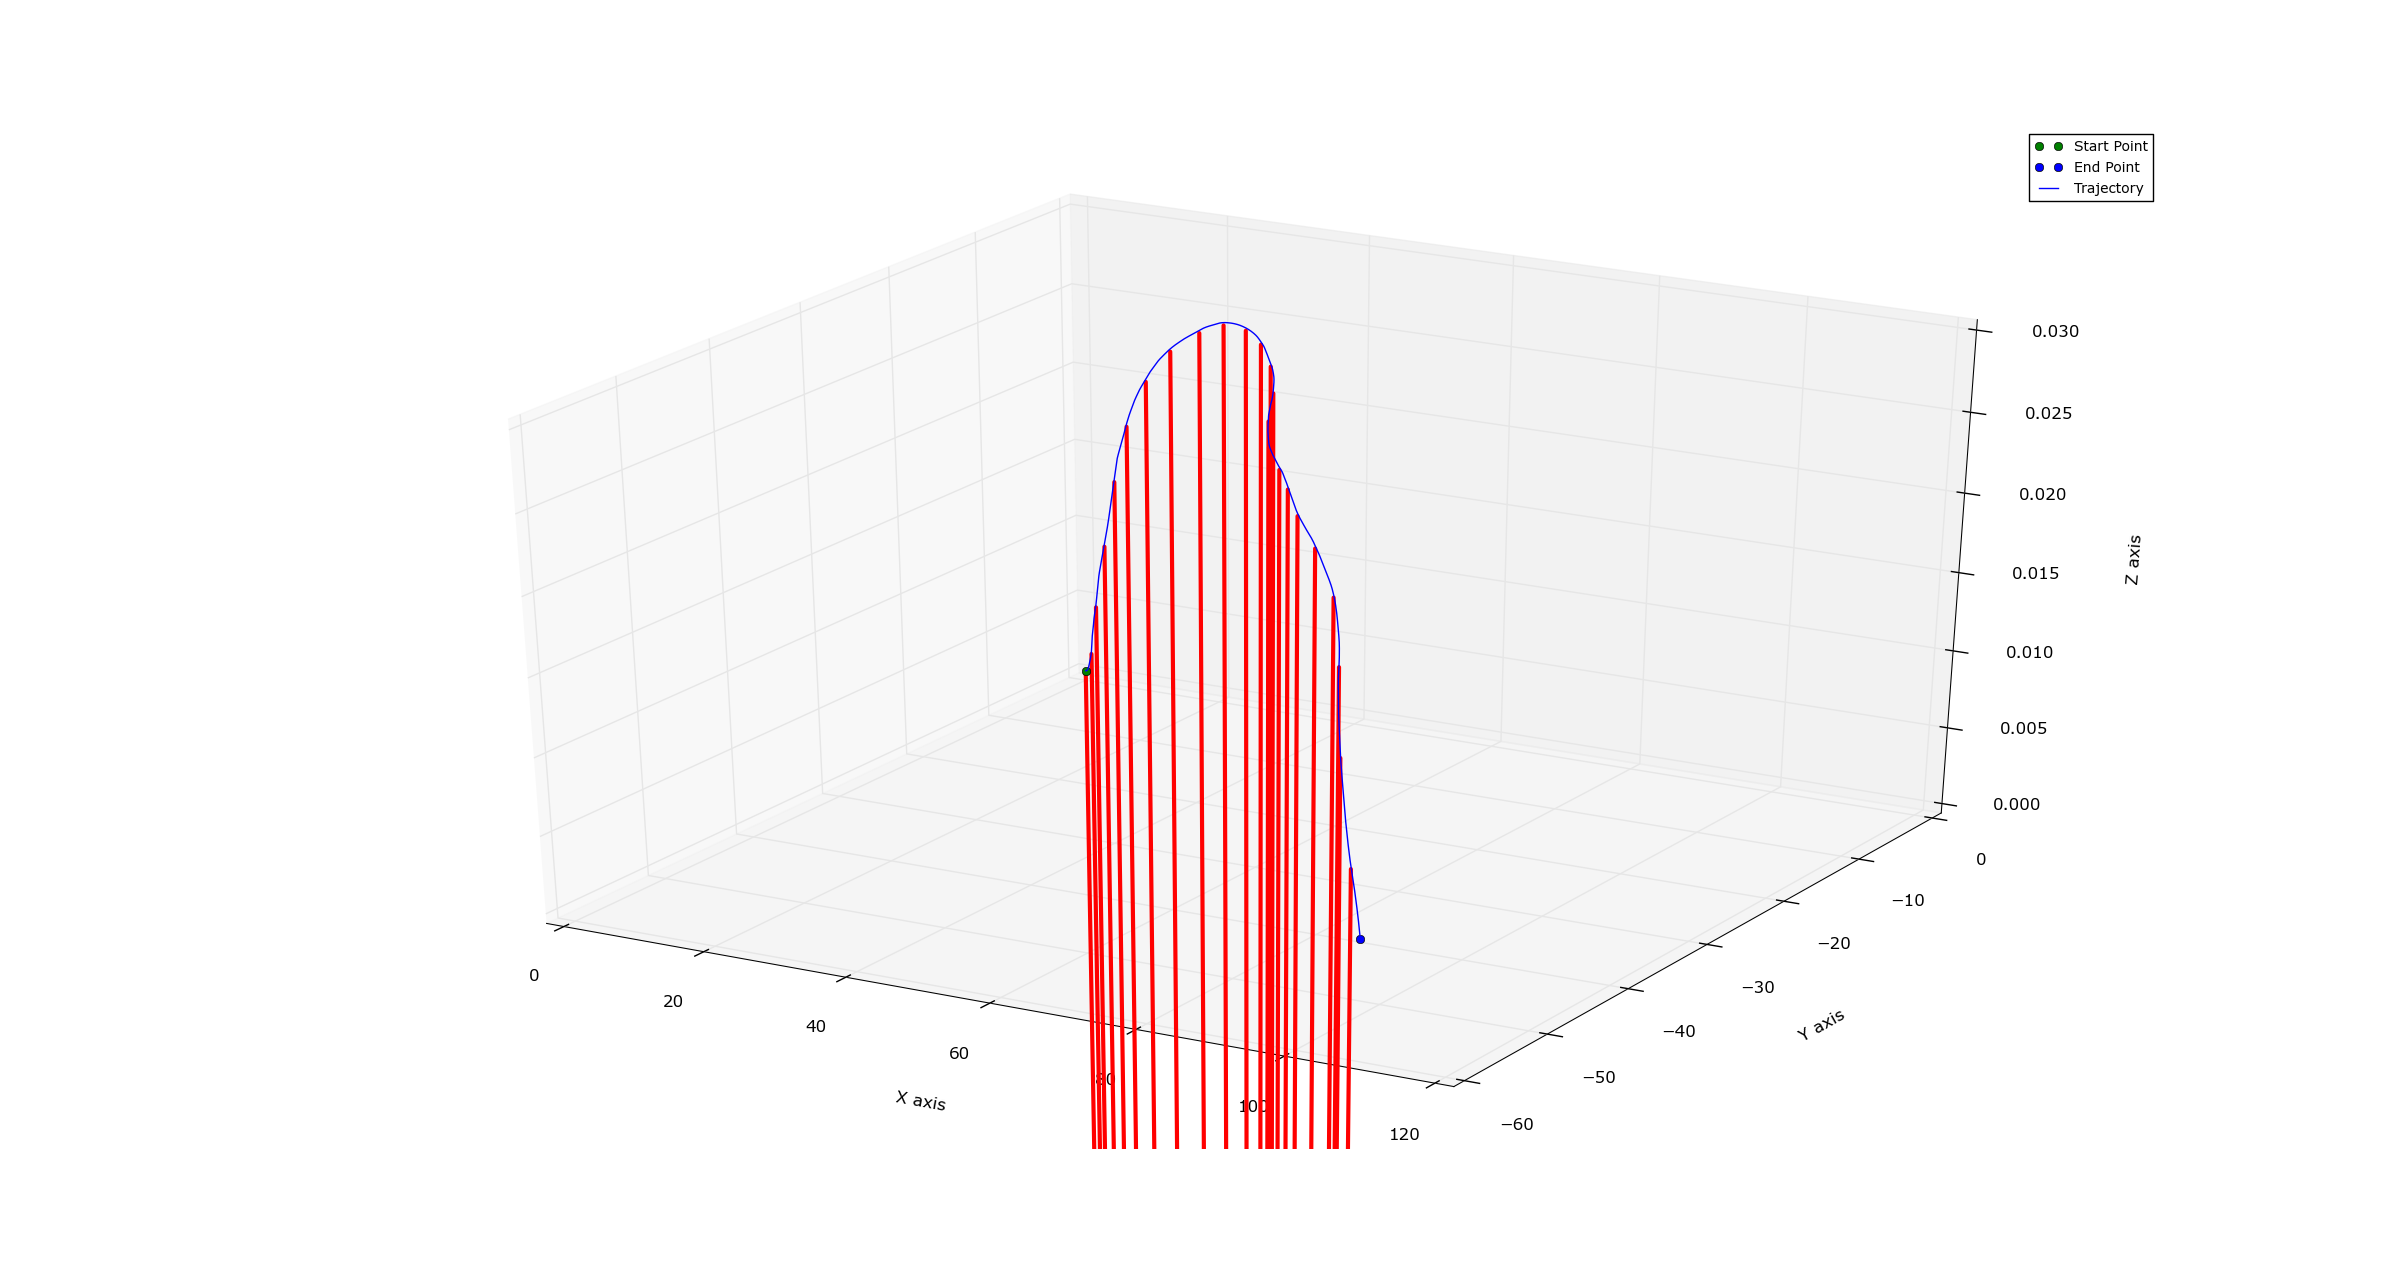
\includegraphics[width=0.4\textwidth]{CONTENT/Figure/Figure5-1a.png}
%		\label{fig:fig5-1-a}}
%	\end{subfloat}\qquad
%	\begin{subfloat}[Trajectory 004]{
%		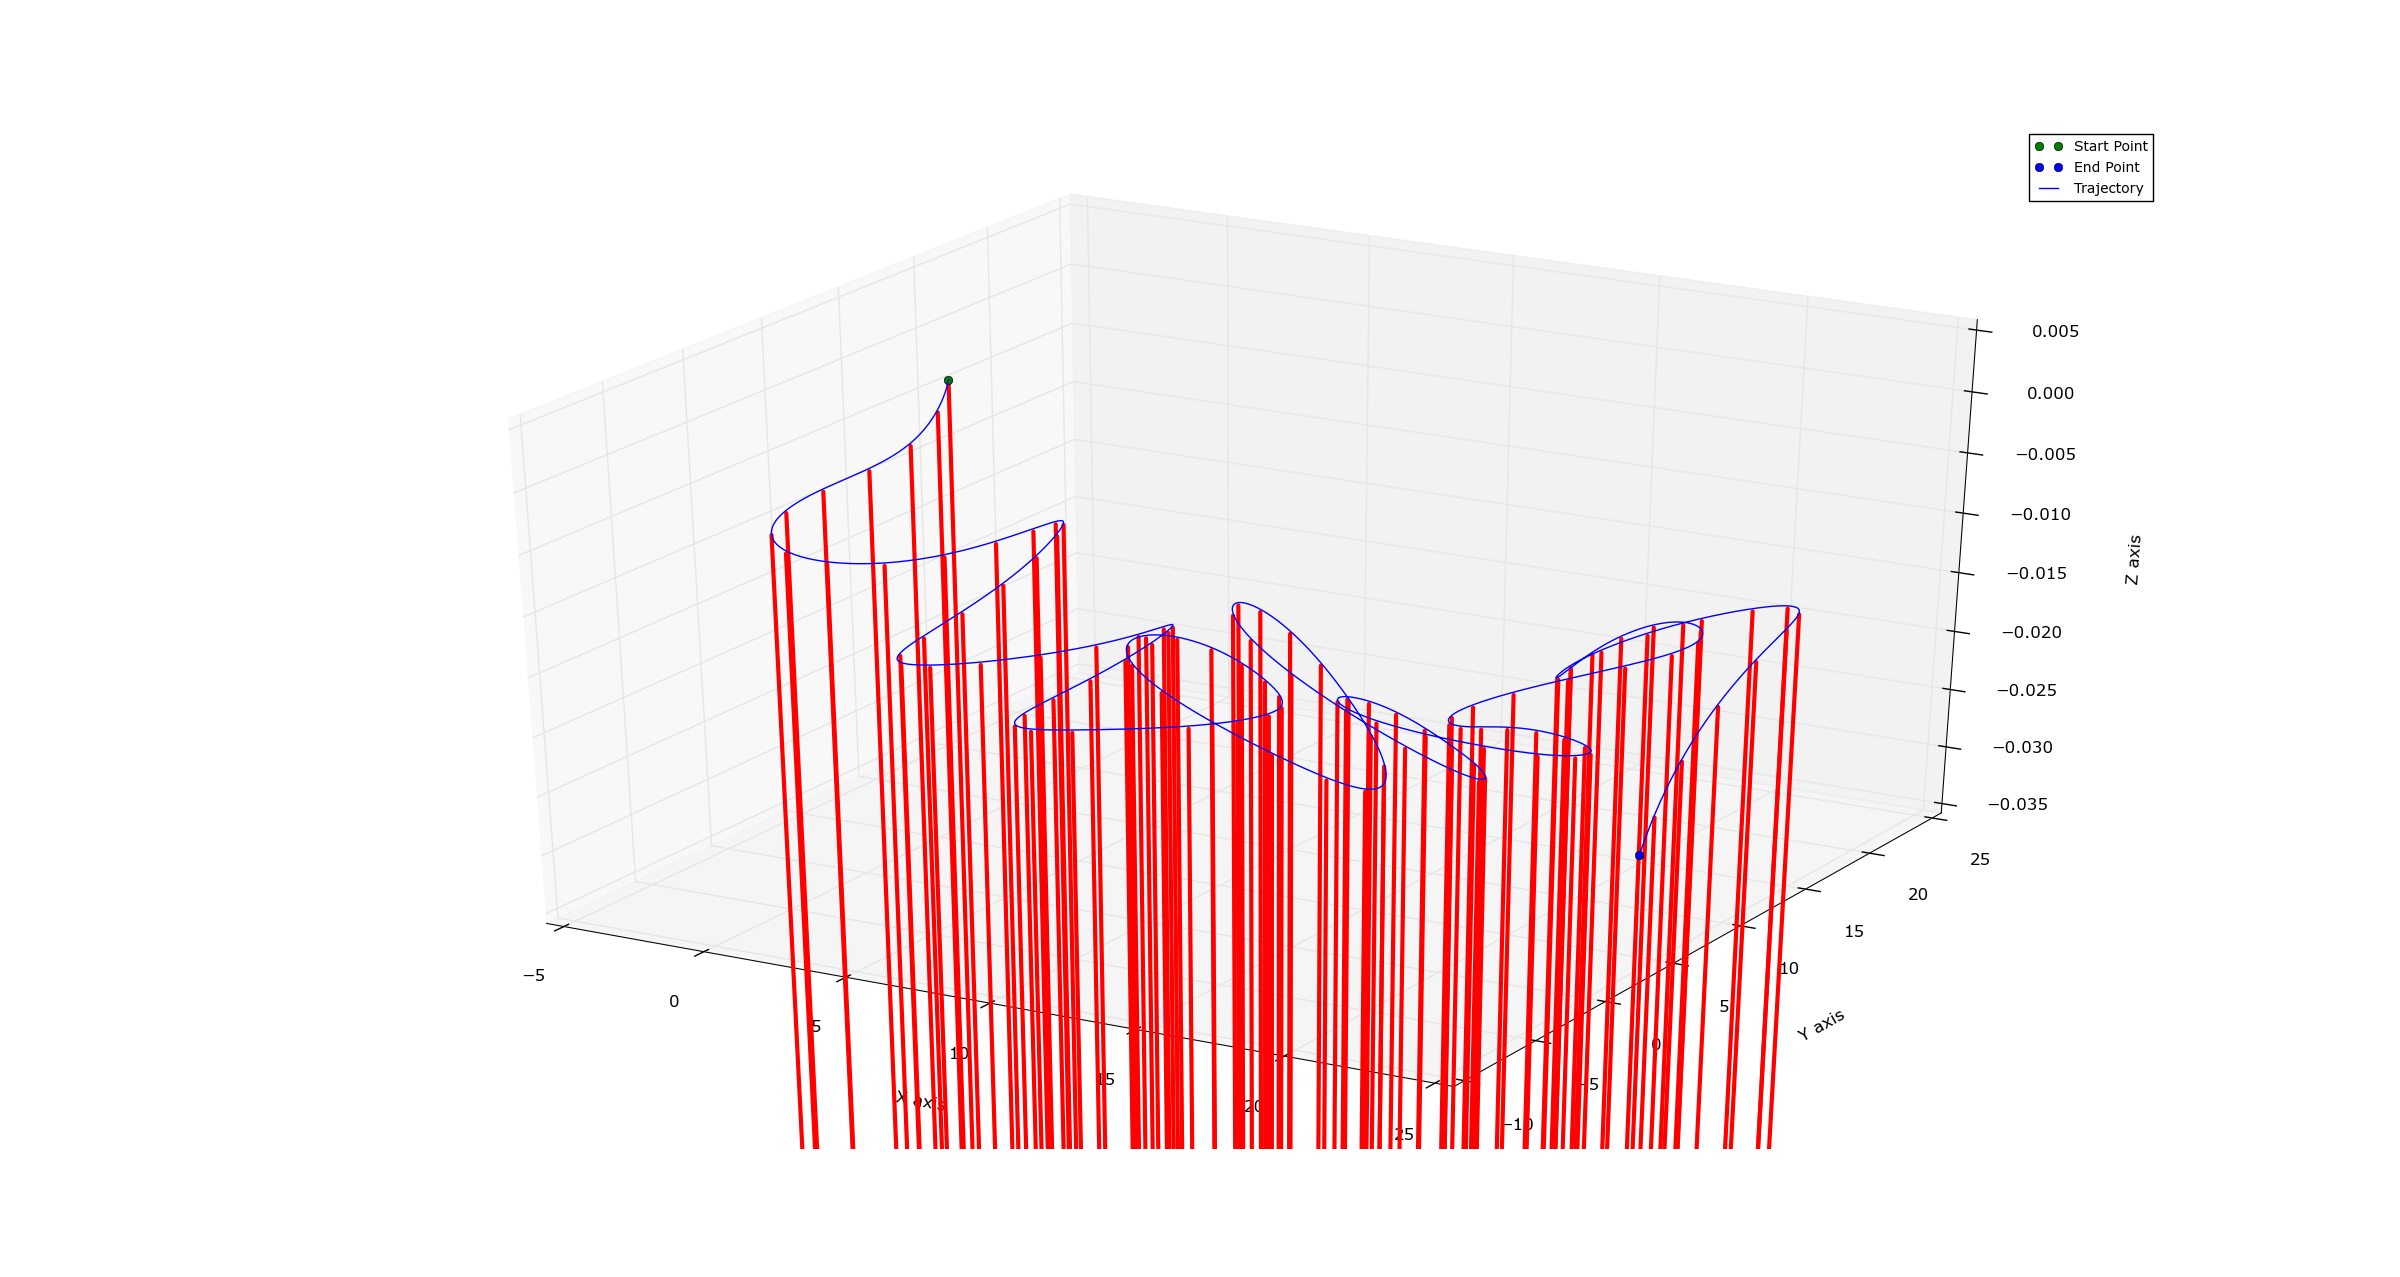
\includegraphics[width=0.4\textwidth]{CONTENT/Figure/Figure5-1b.png}
%		\label{fig:fig5-1-b}}
%	\end{subfloat}
	
	%\hspace*{\fill} % separation between the subfigures
	
%	\caption{Visualization of trajectory \textbf{003} and trajectory \textbf{004}. } 
%	\label{fig:fig5-1}
%\end{figure}

We use a synthetic IMU-camera dataset in this master thesis because it has following advantages rather than real datasets,
\begin{itemize}
\item {Noises in synthetic dataset is controllable. Though we have considered the noise model in our work, the types of noises in real data varies. Besides, denoising from the IMU sensor is beyond the content of this master thesis. }
\item {Synchronization between IMU and camera is easily to be solved. Though we are able to obtain the output frequency of sensors from datasheet or introduction, it is non-trivial to align visual data and inertial data since the frequency of real sensors might be influenced by many environmental factors. In synthetic data, IMU and camera data is aligned automatically because their outputs are stable and fixed.}
\item {Synthetic data is more flexible. We could generate the special cases, \ie, a pure rotation sequence. It is often hard to create such a sequence in the real platform.}
\item {Synthetic data can provide accurate ground truth data \textbf{at each timestamp}. In real platform, a evaluation of position drift usually only happens at end point, \eg, measuring the drift by setting the start point as same as end point. Though a motion capture system is supposed tp provide ground truth data at each timestamp, accuracy of such system usually might be inadequate, and the cost is expensive.}
\item {Numerous calibration steps are saved. In real equipment, it is quite usual to calibrate the device again after several uses. We can ignore the calibration processes in simulated platforms.}
\end{itemize}
Also to best of our knowledge, there is no open sourced IMU-camera synthetic dataset until the writing of this thesis, therefore we decide to generate our own IMU-camera synthetic datasets.

\

\textbf{Trajectory} We start to generate synthetic visual-inertial data by first defining the trajectory of our IMU-camera platform. In VIOs the transformations between the camera sensor and IMU sensor is fixed and pre-calibrated, we assume the camera and IMU sensor share an identical pose in all our experiments for simplification. We have created four different trajectories shown in Table \ref{table:tb1}. Dataset \textbf{001} and Dataset \textbf{002} are used to evaluate the performance of ESKF IMU integration, therefore we apply ground-truth data in \textit{correction step}. Dataset \textbf{003} and Dataset \textbf{004} both evaluate the performance of visual-inertial odometry except \textbf{004} has longer travelled distance and more general shape. There are several general assumptions we have made for simulated trajectories, which are
\begin{itemize}
\item{We assume the initial position of trajectory as $(0, 0, 0)$ in global frame, and initial orientation as quaternion $(1, 0, 0, 0)$ which points at the positive z axis of global coordinate system.}
\item{We assume the second derivative of position and orientation remains constant within two successive sensor samplings.}
\item{We assume the second derivative of position and orientation obeys a normal distribution with additional white Gaussian noise.}
\end{itemize}

\

\textbf{Synthetic IMU data} IMUSim \cite{young2011imusim} is the major tool to simulate IMU data with our customized trajectory. IMUSim is a powerful python-based open-sourced IMU simulation tool, which models a wide range of real-world environments with feasible external noises. To obtain more realistic IMU data, we set the output frequency of IMU as 100 [Hz], sensitivity of gyroscope to 1200 [deg/s] and sensitivity of accelerometer to 4 gravity. The IMU measurements are modelled with the additional white Gaussian noise. Overall we have 3-vector gyroscope readings, 3-vector accelerometer readings, 3-vector ground truth position, 4-vector ground truth orientation from IMUSim for single IMU sampling.

\

\textbf{Synthetic visual data} We simulate virtual scene by Blender \cite{wiki:blender}. We exploit high-frequent grass-like textures and sun lights to simulate the realistic outdoor environment. Thanks to Python interface of Blender, we can import our defined trajectory, and then render a video clip as our visual data set. Here we use linear interpolation for position, \eg, a position $\vec{p}$ between two successive ground truth positions $\vec{p}_t$ and $\vec{p}_{t+1}$ can be computed as
\begin{align}
	\label{e1}
	\Delta{t} &= \frac{t_p - t}{t_1 - t} \\
	\vec{p} &= \vec{p}_t + (\vec{p}_{t+1} - \vec{p}_{t})\Delta{t}
\end{align}
, where $t_p$, $t_1$ and $t$ is time when $\vec{p}$, $\vec{p}_t$ and $\vec{p}_{t+1}$ have been measured. We use \textit{Slerp} to interpolate between two quaternions $\vec{q}_t$ and $\vec{q}_{t+1}$ using Equation (\ref{e1}), we obtain the result $\vec{q}$ as
\begin{align}
	\vec{q} &= \frac{\vec{q}_{t}\sin{((1-\Delta{t})\theta)}+\vec{q}_{t+1}\sin{(\Delta{t}\theta})}{\sin{\theta}}
\end{align}
, where $\theta$ is the half angle between $\vec{q}_t$ and $\vec{q}_{t+1}$. 

The resolution of image is $752 \times 480$, and intrinsic matrix of our virtual pin-hole camera is pre-defined, which is showed in Table \ref{table:tb2}. The output frequency is set to 25 [Hz], three times less than output frequency of the IMU sensor.

\begin{table}[t]
\centering
\begin{tabular}{|c || P{1cm} | P{1cm} | P{1cm} | P{1cm} | P{1cm} | P{1cm} | P{1cm} | P{1cm} | P{1cm} |} 
\hline
 Dataset & fx & fy & cx & cy & d0 & d1 & d2 & d3 & d4 \\
 \hline
 003 & 315.5 & 315.5 & 376.0 & 240.0 & 0.0 & 0.0 & 0.0 & 0.0 & 0.0\\ 
 004 & 315.5 & 315.5 & 376.0 & 240.0 & 0.0 & 0.0 & 0.0 & 0.0 & 0.0\\ 
 \hline
\end{tabular}
     \caption{Intrinsic matrix is only set for trajectory \textbf{003} and \textbf{004} since visual data is not required for trajectory \textbf{001} and \textbf{002}. We use the similar annotation for intrinsic matrix as in \cite{sturm12iros}. The parameter settings are similar with default ROS camera \cite{quigley2009ros}.}
    \label{table:tb2}
\end{table}

\section{Experimental Results}
\label{sec:experiment}

\subsection{Implementation Details}
\label{subsec:imple_detail}

Our implementation consists of a visual odometry based on SVO \cite{forster2014svo} and a loosely-coupled ESKF framework. The goal of visual odometry is to track landmarks (for keyframe BA), estimate camera poses, and select keyframes as we discuss in Section \ref{sec:camera_comple_data}. ESKF framework aims to integrate IMU measurements over timestamps, and fuse the visual results in correction step.

SVO \cite{forster2014svo} is a fast semi-direct monocular visual odometry. Instead of applying image features, the camera pose is estimated by minimizing photometric errors between successive images. SVO is very efficient because the high-cost feature extraction step has been skipped, besides a probabilistic mapping method has been used, therefore more reliable 3D landmarks can be obtained. Overall SVO provides a efficient and robustness way to obtain camera poses, keyframes and 3D landmarks. 

We implement C\texttt{++} based ESKF framework as we explain in Section \ref{sec:ESKF_IMU}. Mathematical operations such as quaternion operations, and matrix operations are implemented with efficient C\texttt{++} template linear algebra library Eigen \cite{eigenweb}. In keyframe BA part, the basic BA solver is provided by Google Ceres Solver \cite{ceres-solver}, we select the maximum number of keyframes to 20 for efficiency reasons, the BA step runs in parallel with ESKF. IMU measurements has been already aligned with visual measurements initially and manually (every four IMU data corresponds to one image frame).

All experiments are processed with a Intel Core i7 4700MQ laptop, and all codes related to this master thesis will be published on \url{https://github.com/OscarLiXi/MasterThesis} afterwards.

\subsection{Experiment 1: IMU Integration}
\label{subsec:experiment1}

In this experiment, we examine the correctness and efficiency of single IMU integration (without extrasensory correction data). Since \textbf{001} and \textbf{002} are special cases that many VO system \cite{davison2003real, engel2014lsd} have failed, and dataset \textbf{004} is a general simulated micro helicopter trajectory, these three datasets are applied in this experiment to show the correctness of our IMU integration. Moreover we assume the VO provides us a very accurate camera pose estimation in correction step at a lower rate.  

We have reported the results in Figure \ref{fig:fig5-2} and Table \ref{table:tb3}. For trajectory \textbf{001}, the average position drift is approximately 0.125 [m], which is less than 0.08\% of total travelled distance (see Table \ref{table:tb1}). For trajectory \textbf{002}, the average attitude drift is approximately 0.0134 [rad], which is less than 0.8 [deg]. For more realistic and longer trajectory \textbf{004}, the average position drift is larger because error accumulation is inevitable, the average error is less than 0.55\% of overall distance travelled; the results of average attitude error is also acceptable but has larger variance as we can see from Figure \ref{fig:fig5-2-f}. The time for processing a single IMU measurement does not grow as time goes by, which supports our claim that ESKF IMU integration runs under a constant time computational complexity. Furthermore, ESKF needs approximately 0.019 [ms] in a single run, therefore it runs in a real-time considering the output frequency of IMU is 100 [Hz].

We conclude from this experiment that our ESKF IMU integration can deal with normal and special cases, and it has a precise pose estimation results \textbf{if VO system has given a accurate correction}. In next few experiments we will abandon this assumption, and demonstrate some other comparisons. In addition, experimental results show that ESKF IMU runs in real-time, which the computational complexity of single IMU integration remains constant as we point out in Section \ref{sec:pipeline_summary}. 

\begin{figure}
\centering
	\begin{subfloat}[]{
		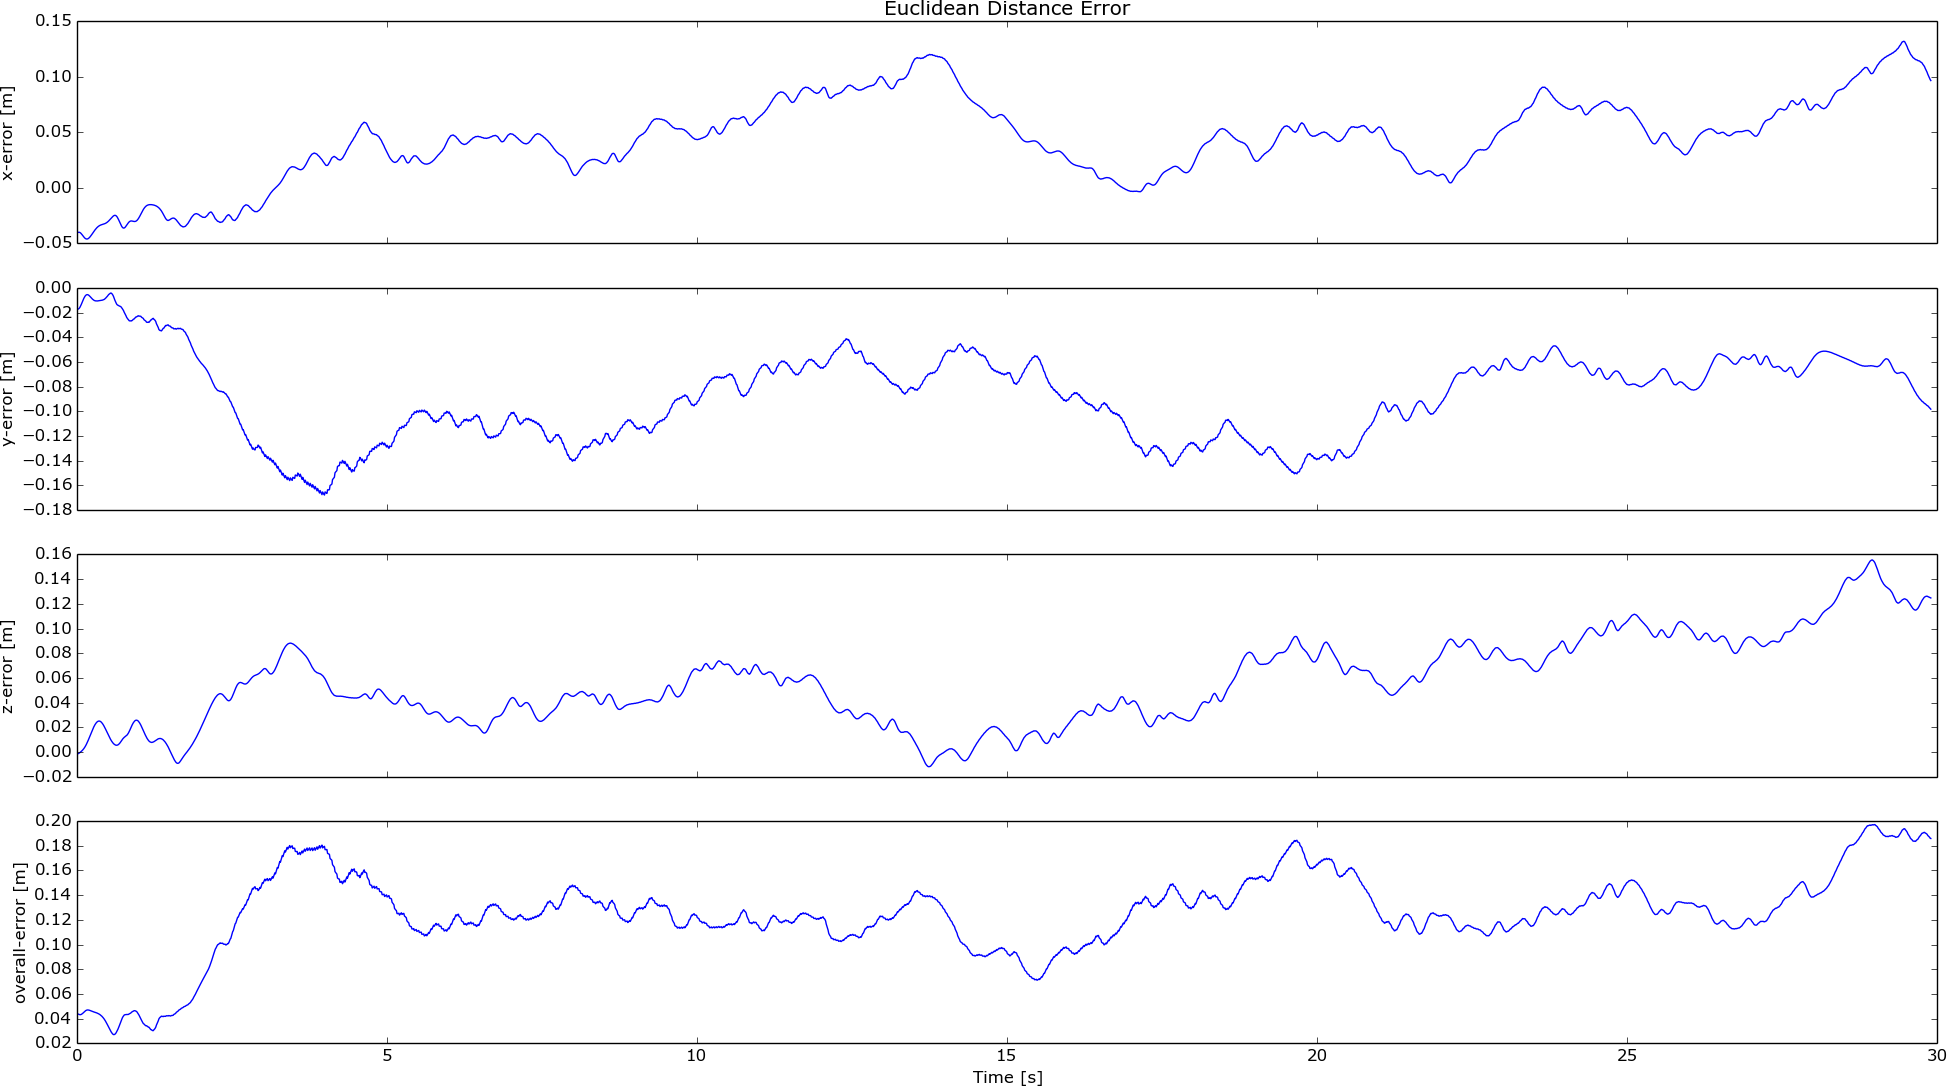
\includegraphics[width=0.45\textwidth]{CONTENT/Figure/figure5_2_a.png}
		\label{fig:fig5-2-a}}
	\end{subfloat}\qquad
	\begin{subfloat}[]{
		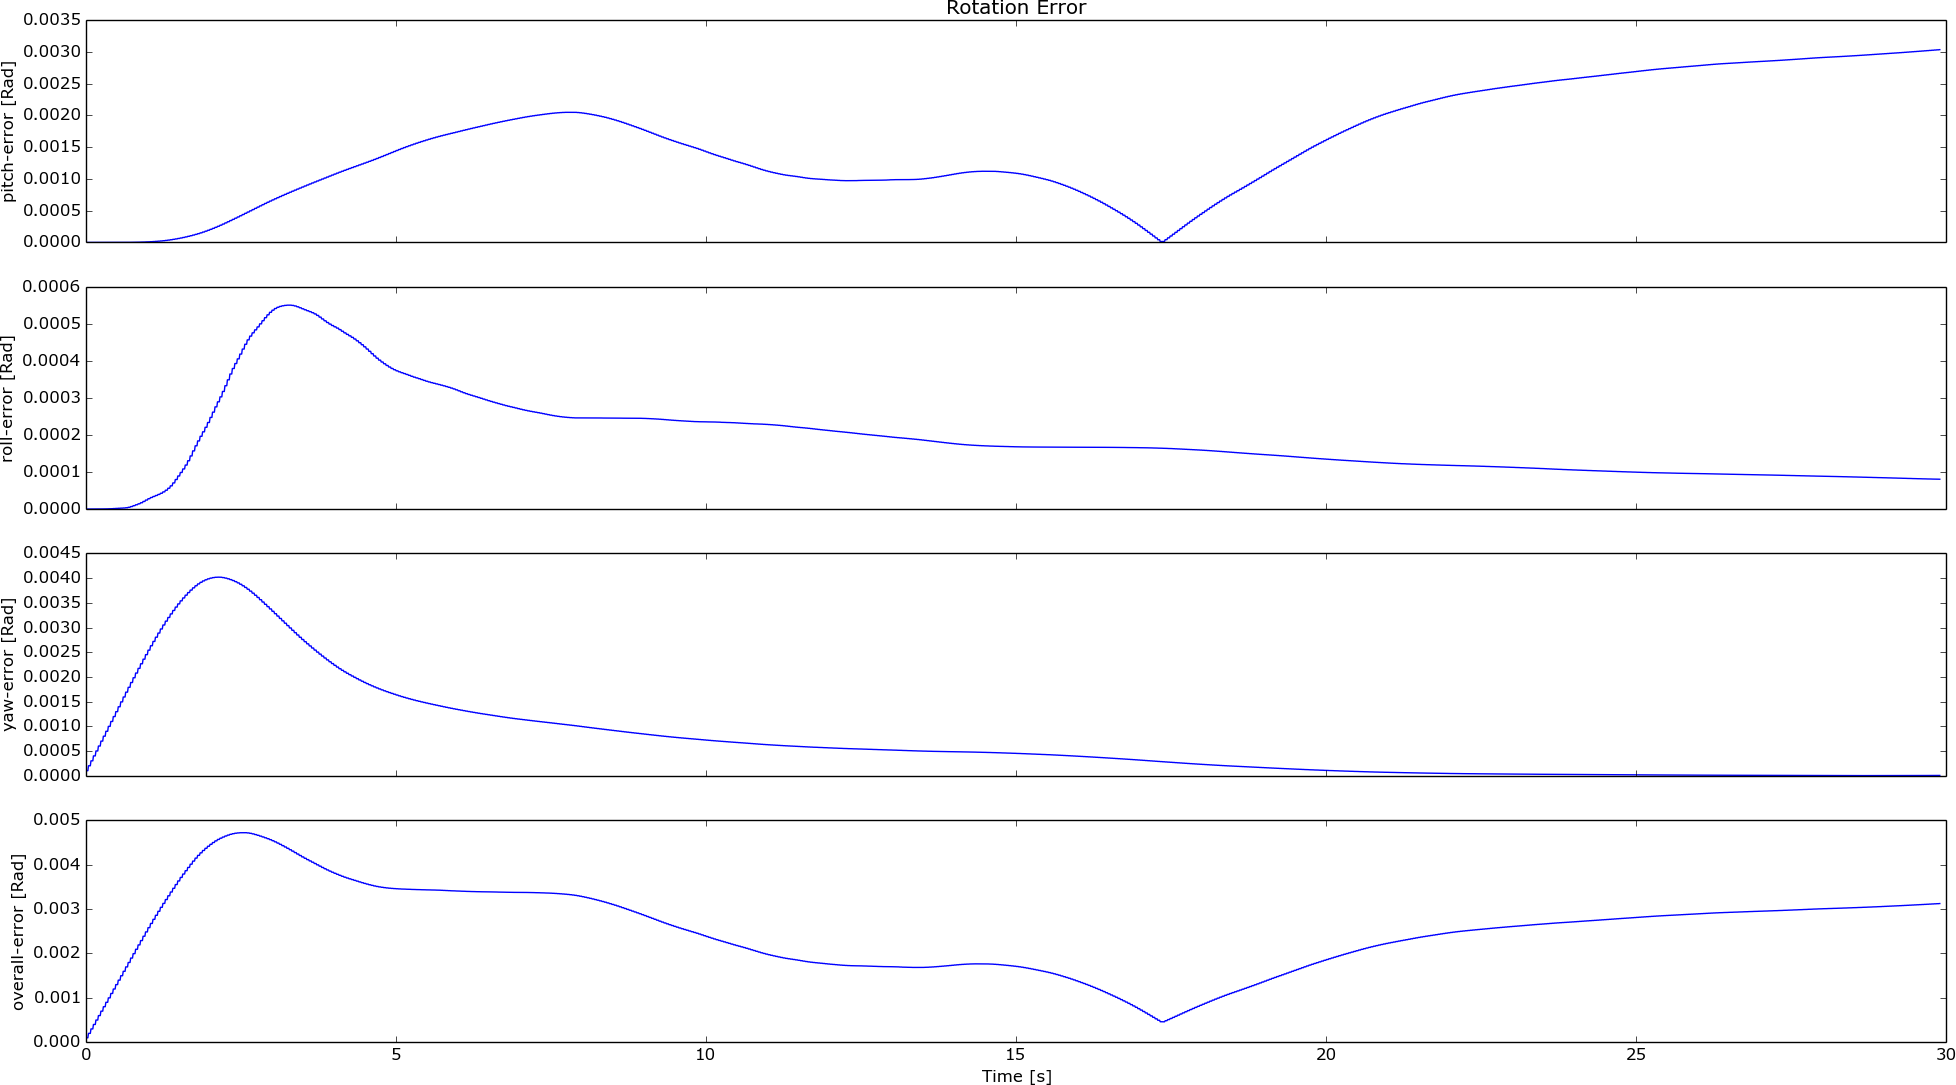
\includegraphics[width=0.45\textwidth]{CONTENT/Figure/figure5_2_b.png}
		\label{fig:fig5-2-b}}
	\end{subfloat}
		\begin{subfloat}[]{
		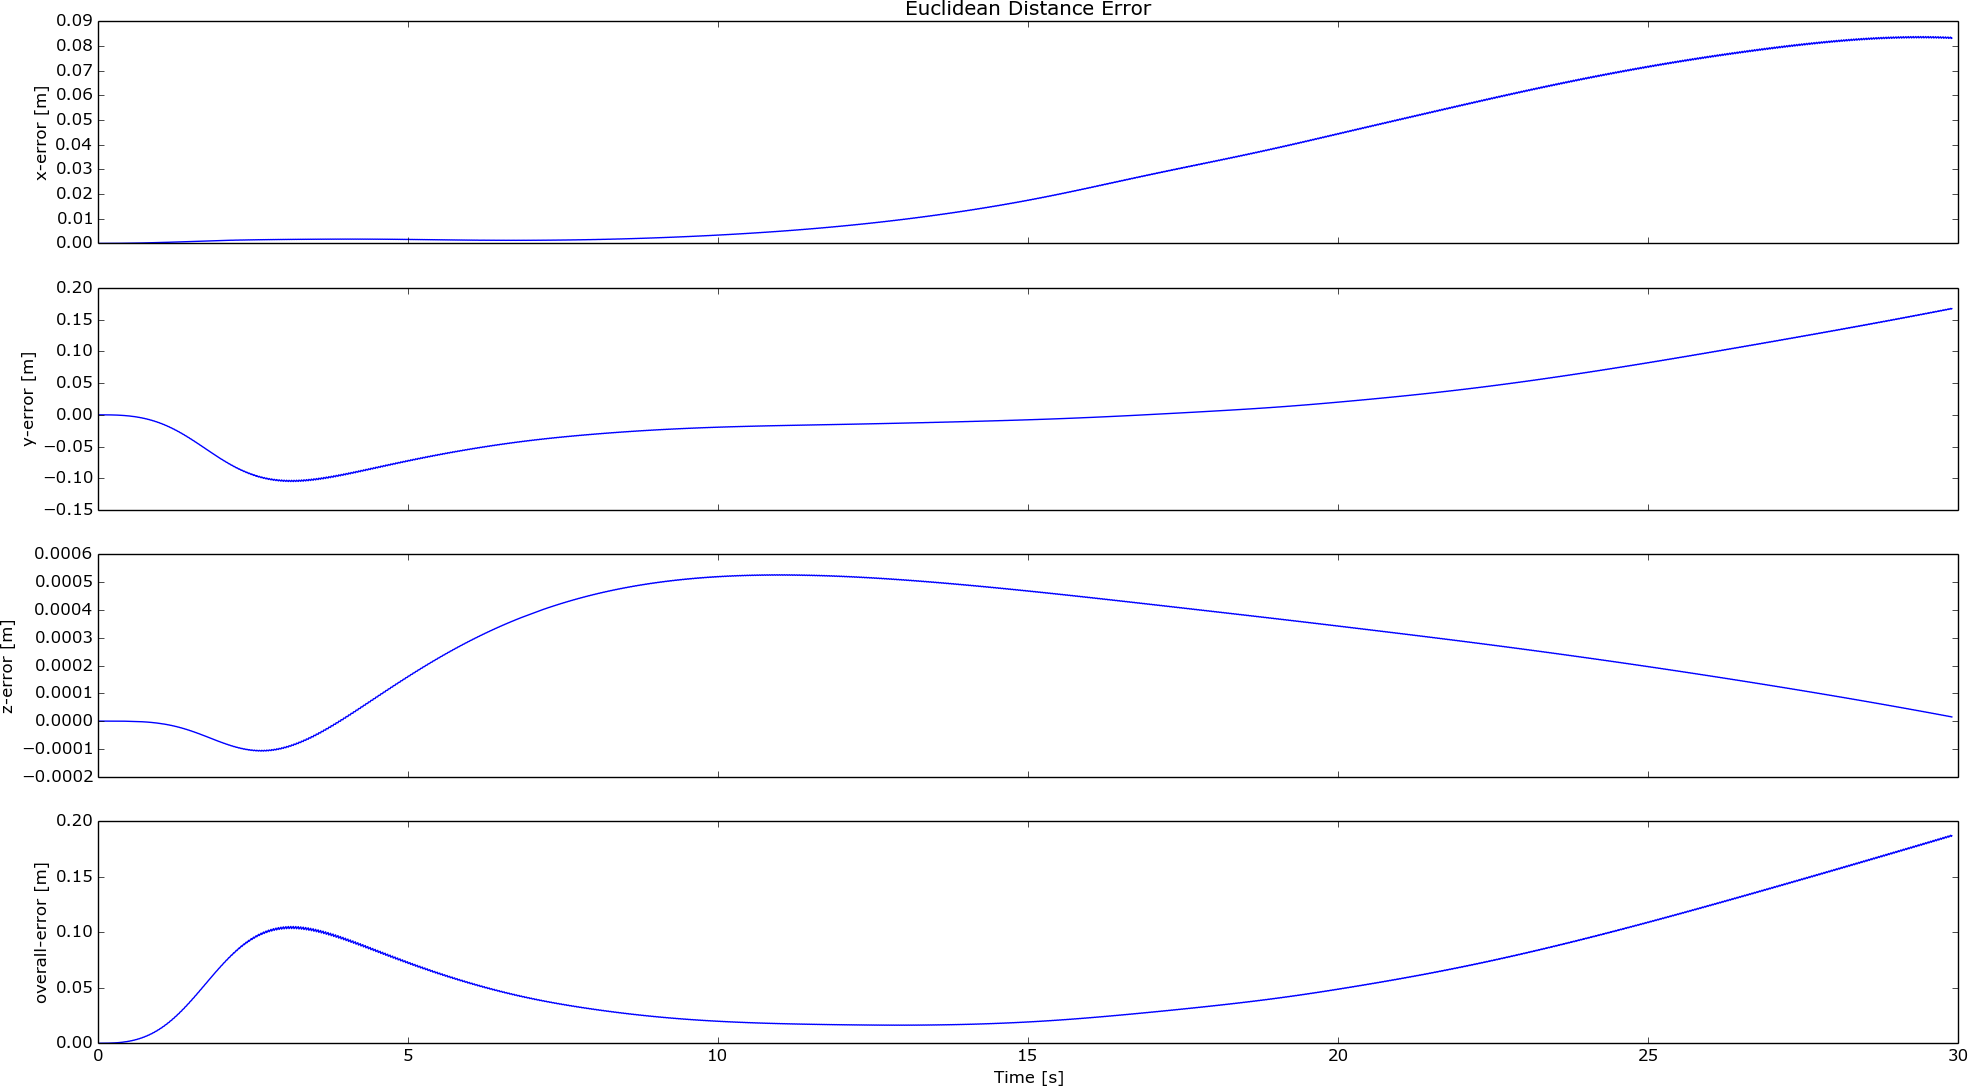
\includegraphics[width=0.45\textwidth]{CONTENT/Figure/figure5_2_c.png}
		\label{fig:fig5-2-c}}
	\end{subfloat}\qquad
	\begin{subfloat}[]{
		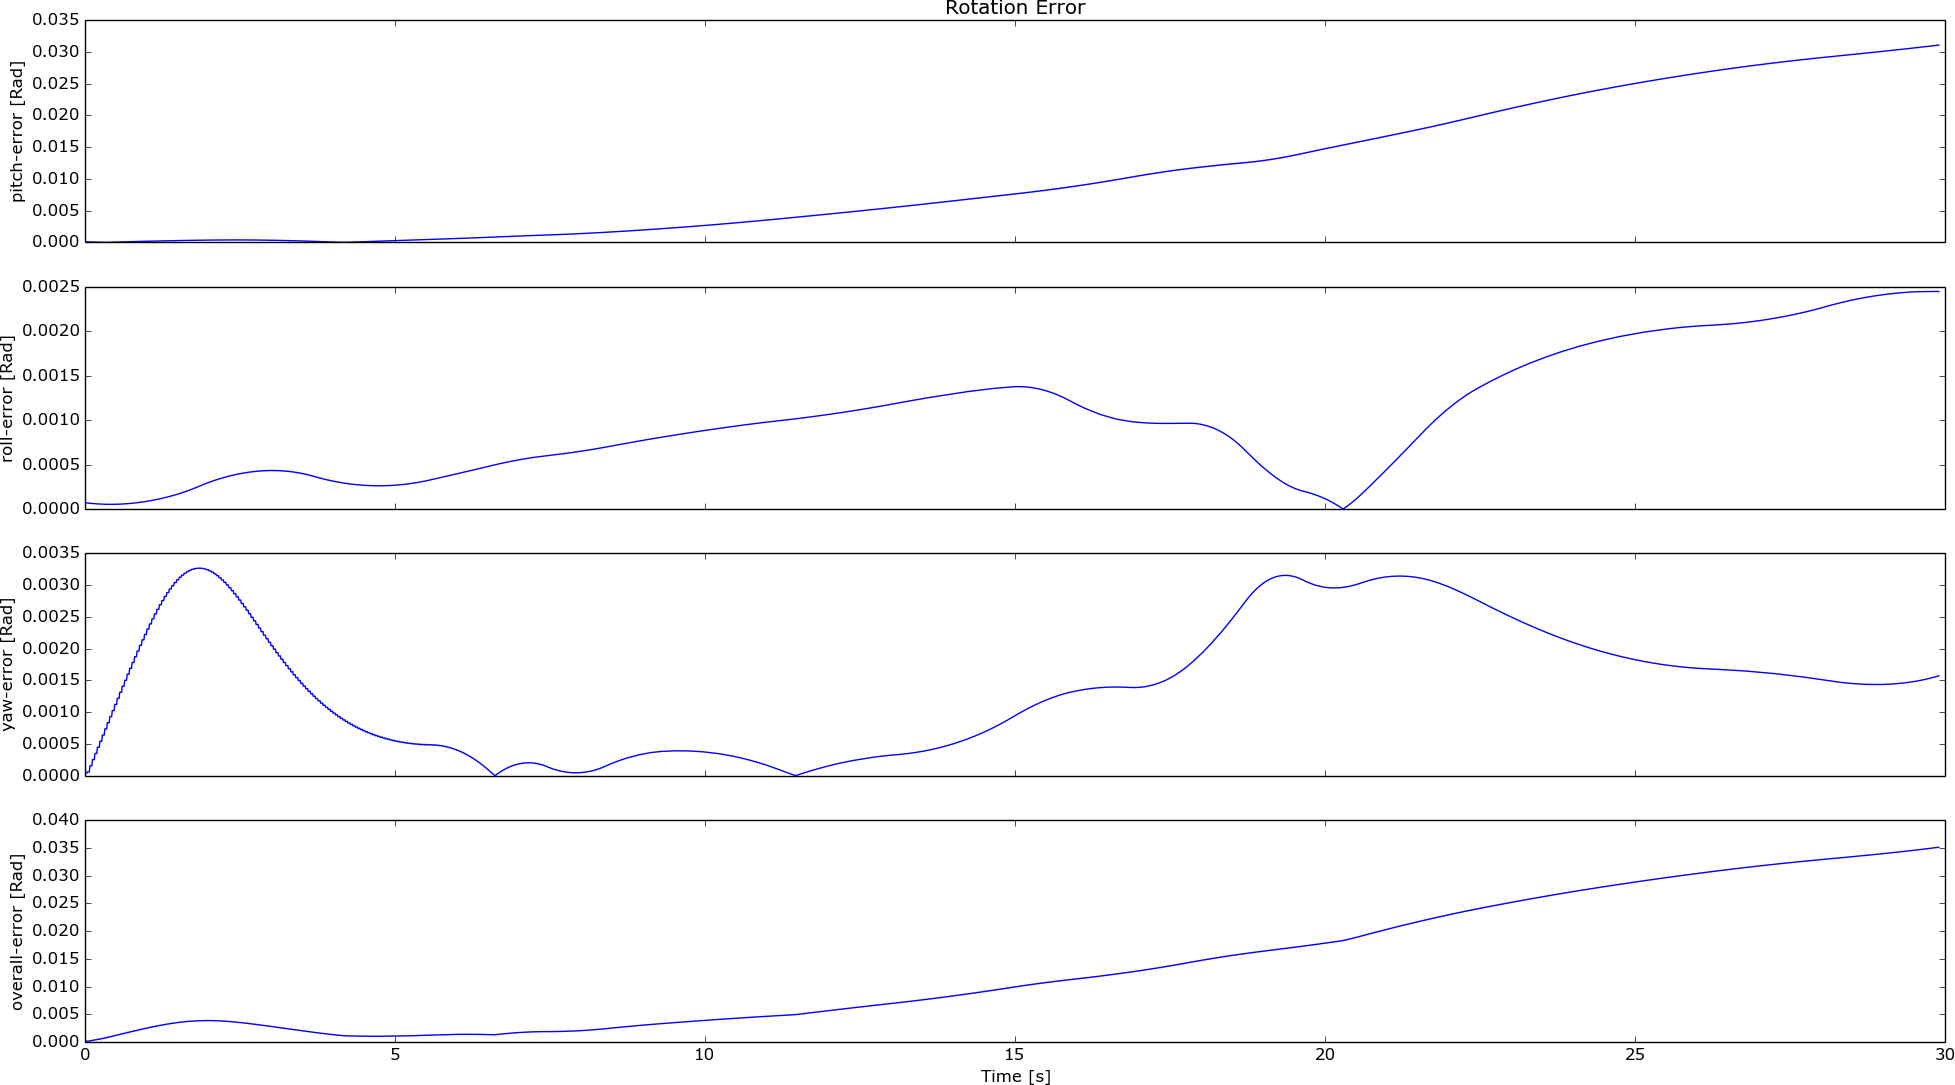
\includegraphics[width=0.45\textwidth]{CONTENT/Figure/figure5_2_d.png}
		\label{fig:fig5-2-d}}
	\end{subfloat}
		\begin{subfloat}[]{
		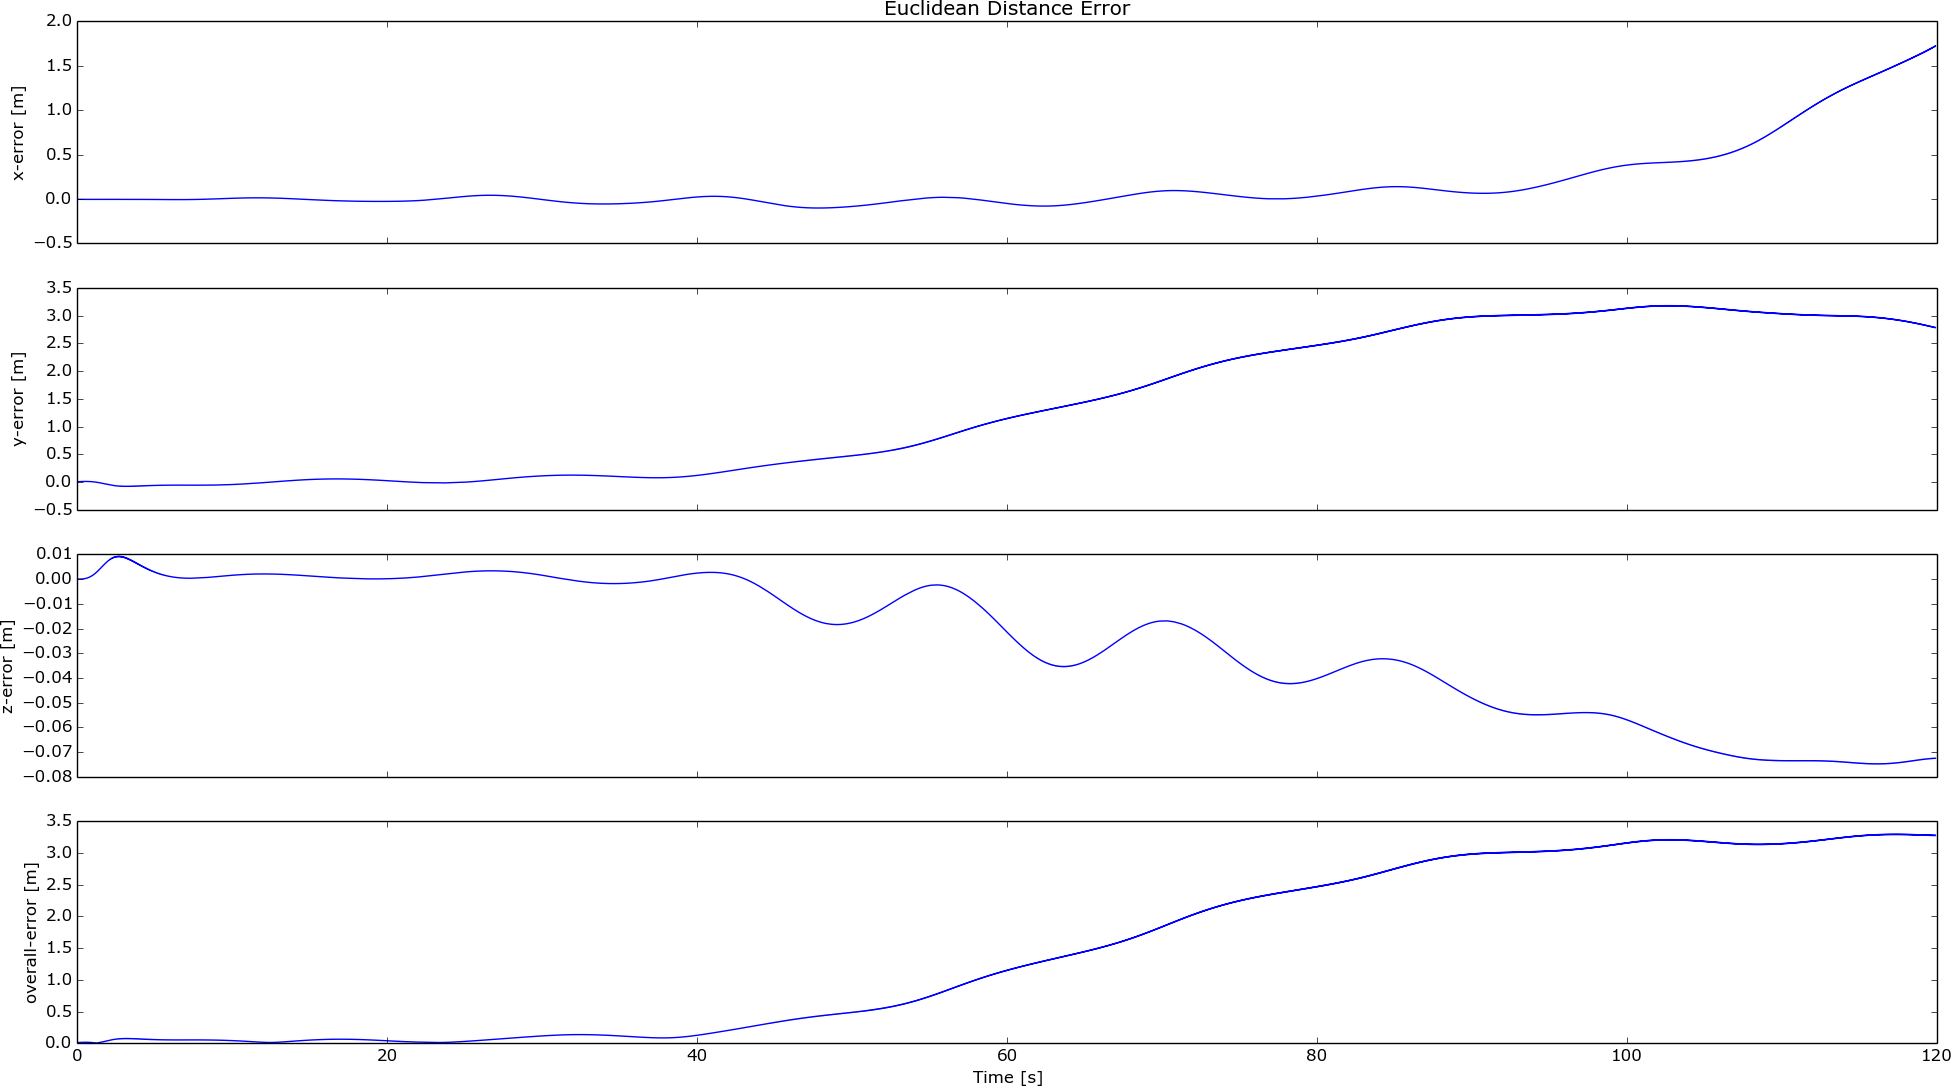
\includegraphics[width=0.45\textwidth]{CONTENT/Figure/figure5_2_e.png}
		\label{fig:fig5-2-e}}
	\end{subfloat}\qquad
	\begin{subfloat}[]{
		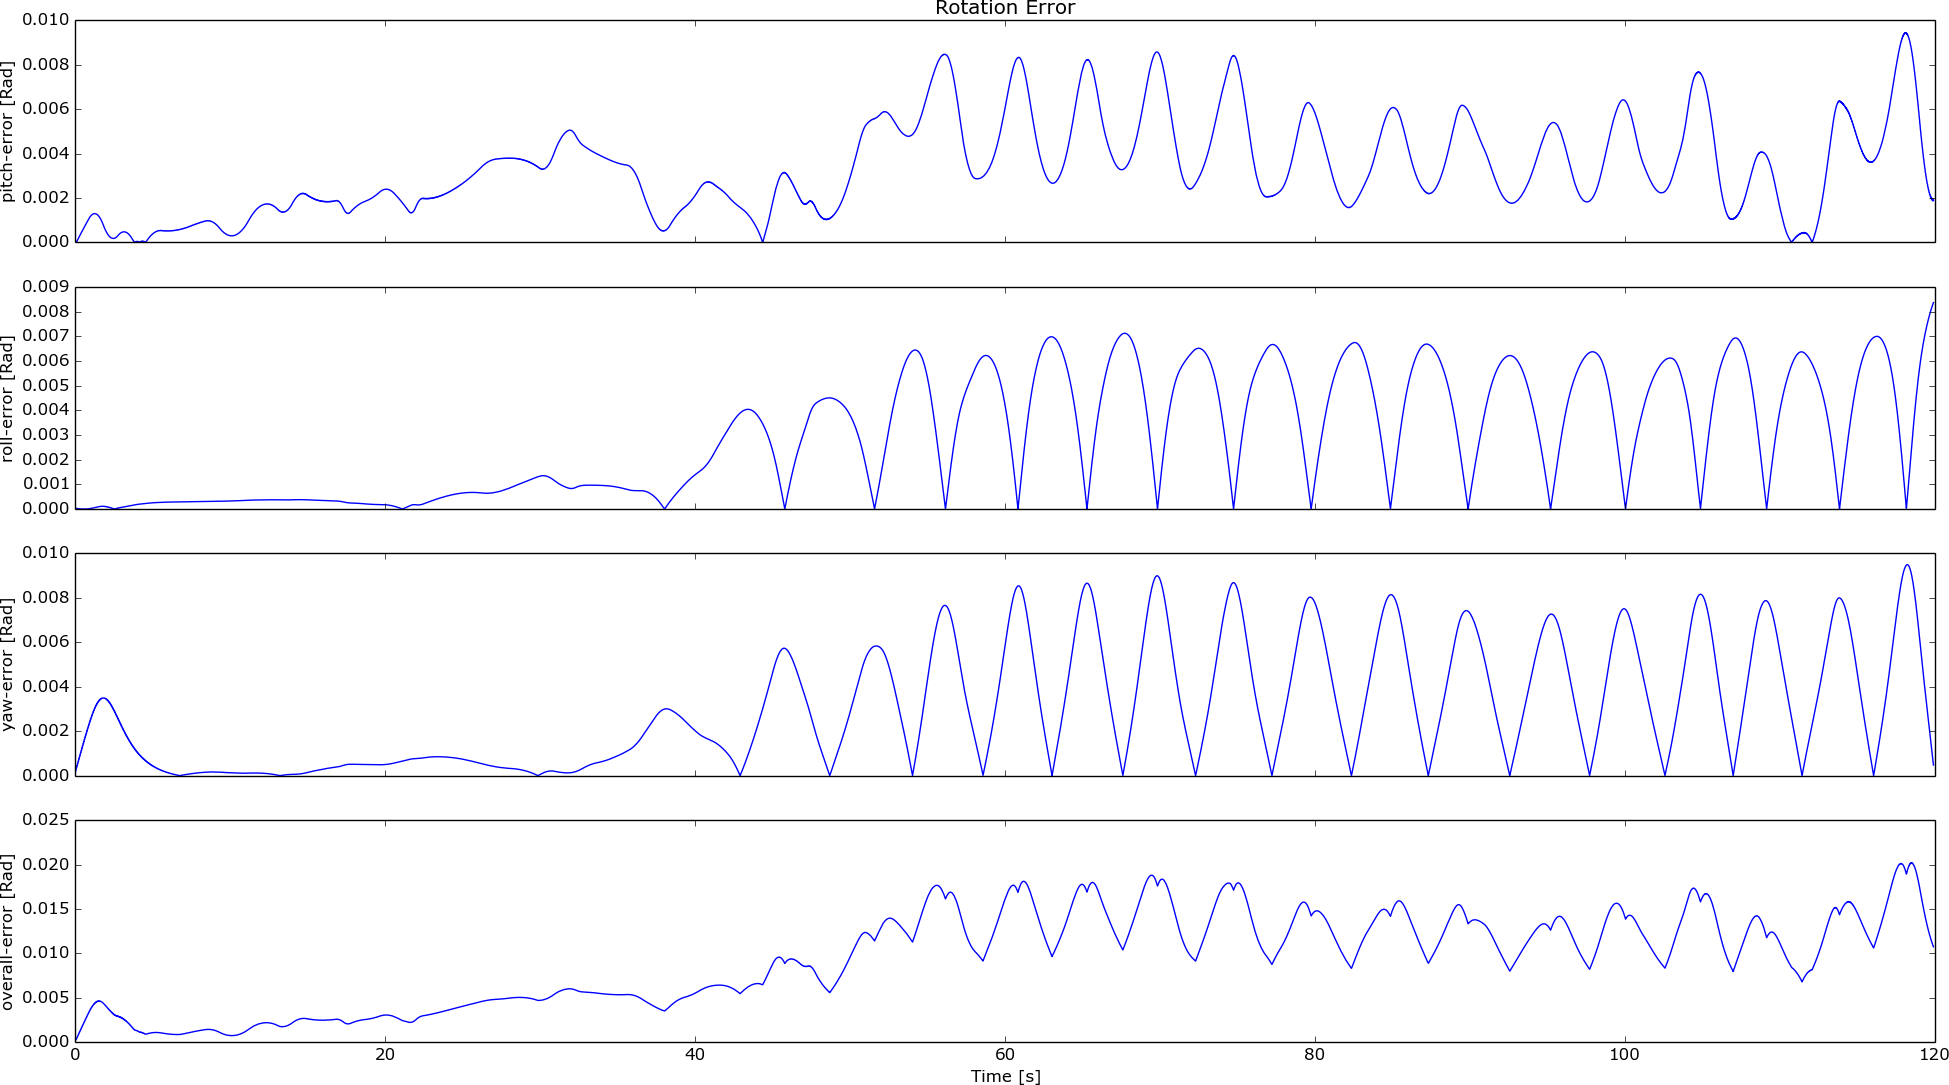
\includegraphics[width=0.45\textwidth]{CONTENT/Figure/figure5_2_f.png}
		\label{fig:fig5-2-f}}
	\end{subfloat}
	
	%\hspace*{\fill} % separation between the subfigures
	
	\caption{Experiment 1: (a)(b) Position and attitude drift of Dataset \textbf{001} (c)(d) Position and attitude drift of Dataset \textbf{002} (e)(f) Position and attitude drift of Dataset \textbf{004}. Position error is measured using Euclidean distance, and attitude drift is measured by transforming quaternion back into Euler angle (see Appendix \ref{chap:appendix3}) since it is more straightforward to evaluation. Ground truth data is provided by synthetic IMU data generator.} 
	\label{fig:fig5-2}
\end{figure}

\begin{table}[t]
\centering
\begin{tabular}{|c || P{3cm} | P{3cm} | P{3cm} |} 
\hline
 Dataset & APD [m] & AAD [Rad] & TPD [ms] \\
 \hline
 001 & 0.1251 & 0.0025 & 0.0184 \\ 
 002 & 0.0622 & 0.0134 & 0.0188 \\ 
 004 & 1.4319 & 0.0094 & 0.0187 \\ 
 \hline
\end{tabular}
     \caption{Experiment 1: APD (Average Position Drift) and AAD (Average Attitude Drift) is measured by averaging overall position and attitude drift. For TPD (Time-elapsed Per Data), we run the experiment 100 times to measure a overall elapsed time, then divide by number of experiments and number of IMU measurements to obtain the single data processing time.}
    \label{table:tb3}
\end{table}

\subsection{Experiment 2: VIO Versus VO}
\label{subsec:experiment2}

In this experiment, we will compare our suggested VIO with single VO using same data sequences. As we have discussed before, correction data by visual sensor has a large impact on our final pose estimation since global translation and angle rotated around gravity vector (yaw) are unobservable for IMU. In loosely-coupled IMU integration, ESKF needs visual results because it is not aware of exact movement model. Here we propose the experiment 2 roughly under the pipeline in Section \ref{sec:pipeline_summary} except we exclude the keyframe BA procedure, which will be added as an extra correction shown in the experiment 3.

The results of experiment 2 on trajectory \textbf{004} have been shown in Figure \ref{fig:fig5-3}. It is clear that VIO has lower variance than VO in translation though they have similar average position drift. VIO has given better results than VO regarding to the attitude drift. The reason is VIO gains much lower error than VO in two observable parameters (pitch and roll), and we can also see that VIO and VO report the similar error curve in yaw. These results are competitive among similar systems \cite{mourikis2007multi, forster2015imu} with similar overall travelled distance. We also evaluate the processing time using similar way as in Section \ref{subsec:experiment1}, VIO finally has an average time per IMU data as 4.570 [ms], which processes the measurements in real-time.

We conclude that the VO has a huge positive impacts on 3-vector global translation and rotational angle around gravity vector. The estimated results by fusing visual data and IMU data has lower variance and higher accuracy than single visual odometry, and undoubtedly single IMU integration.

\begin{figure}
\centering
	\begin{subfloat}[]{
		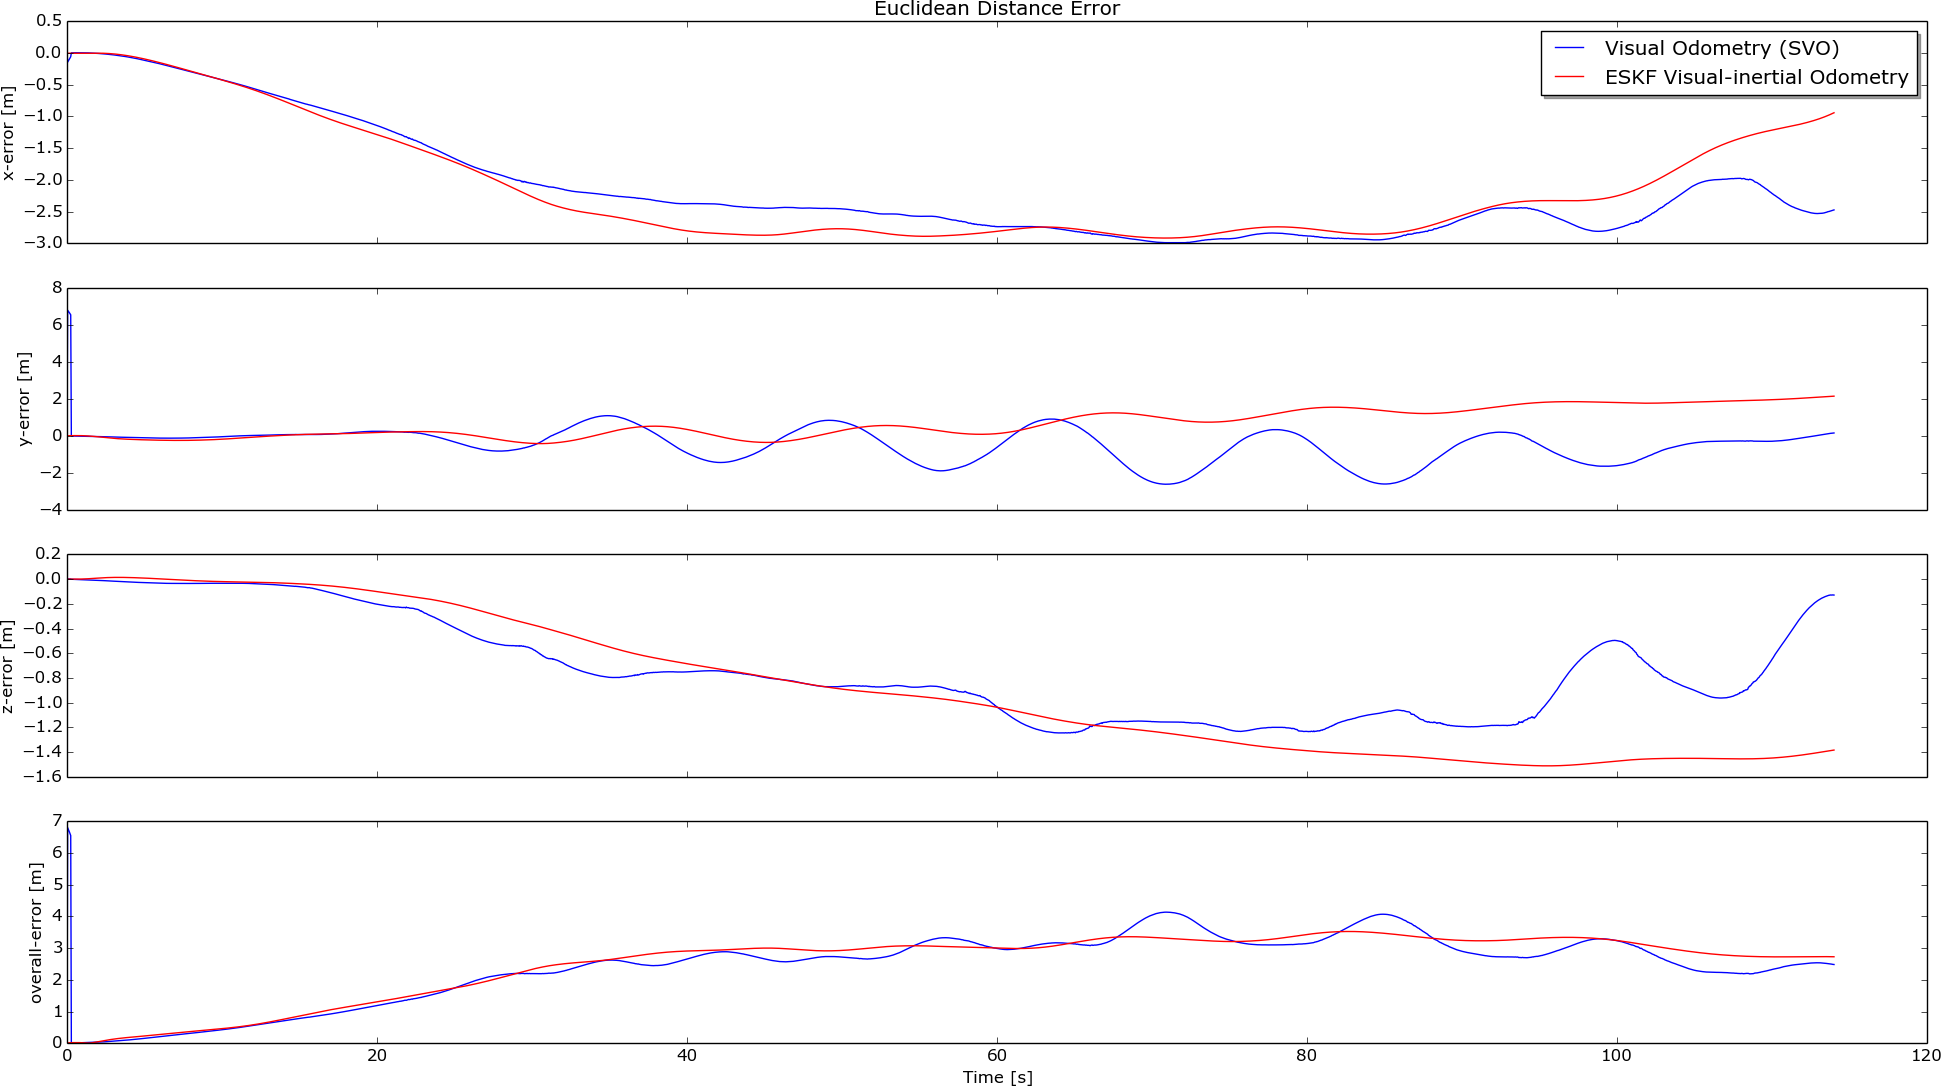
\includegraphics[width=0.45\textwidth]{CONTENT/Figure/figure5_3_a.png}
		\label{fig:fig5-3-a}}
	\end{subfloat}\qquad
	\begin{subfloat}[]{
		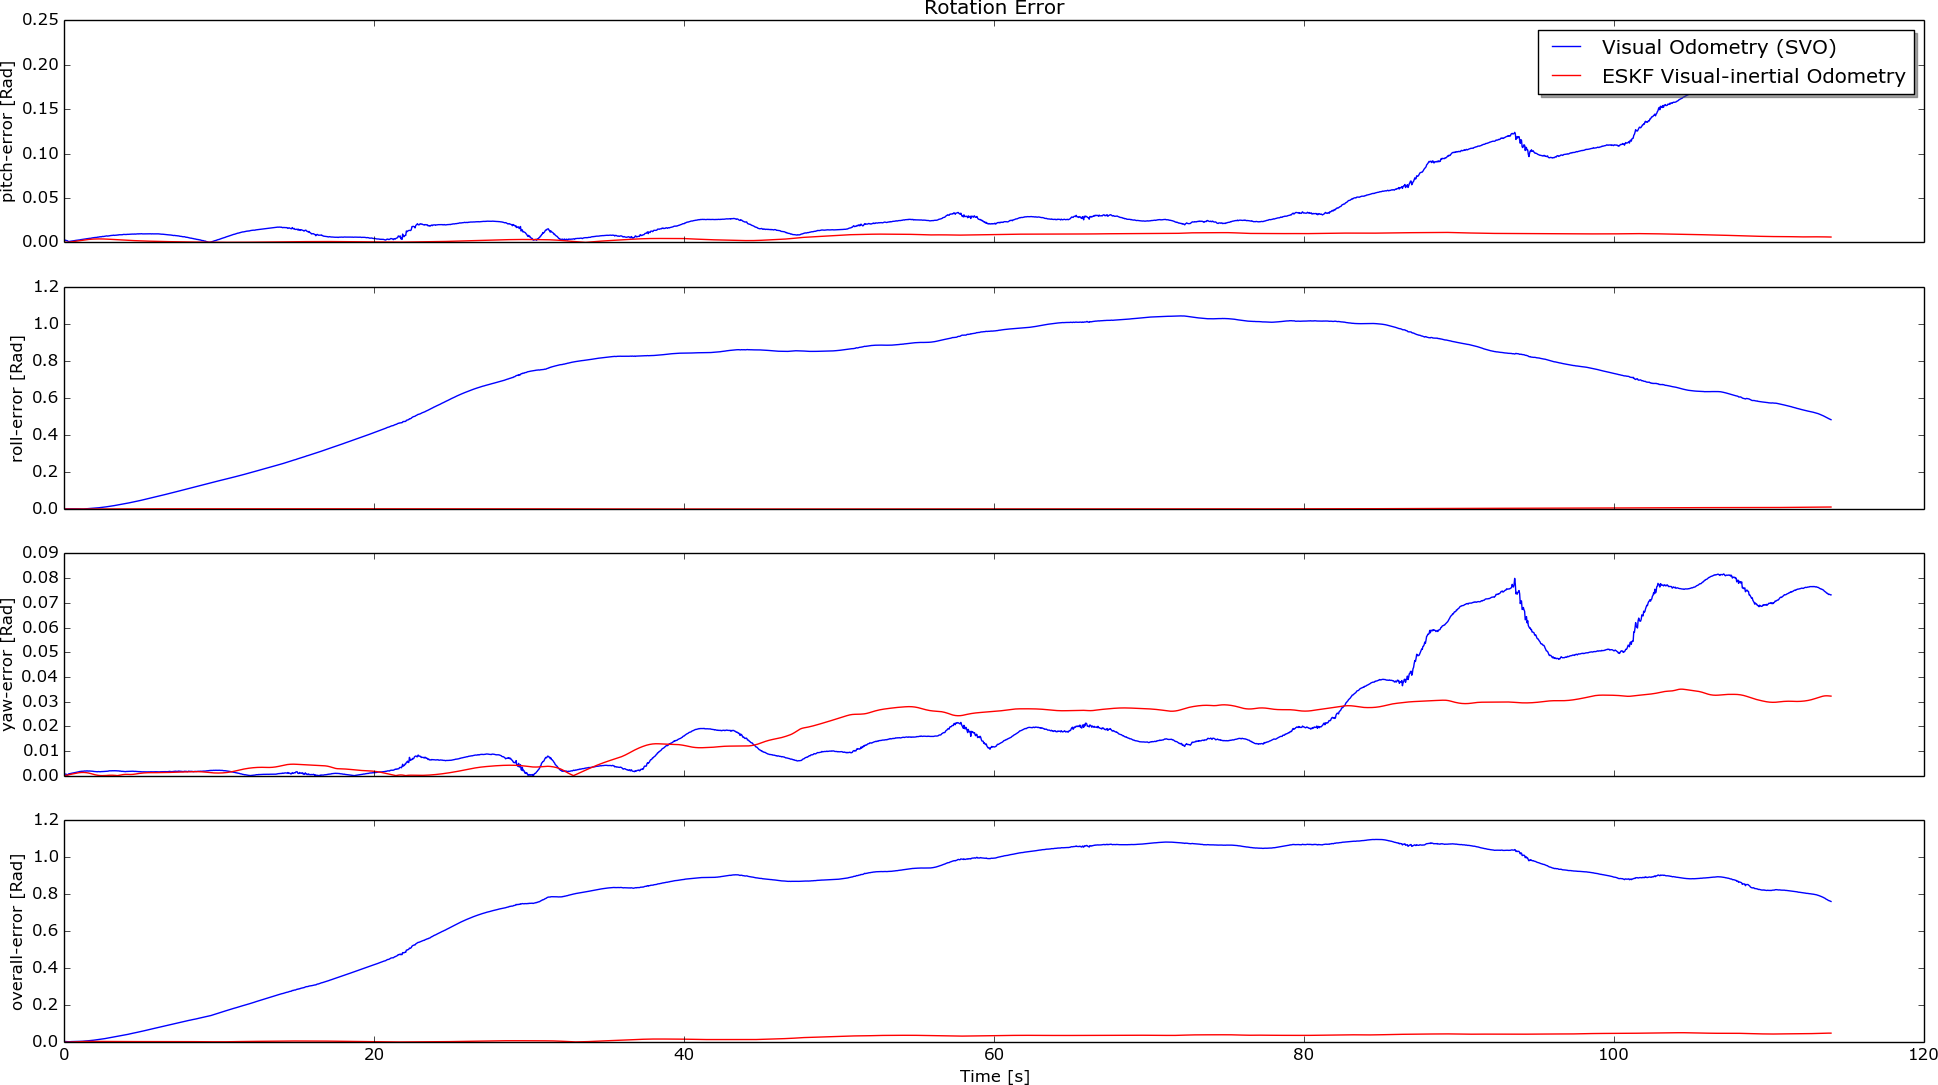
\includegraphics[width=0.45\textwidth]{CONTENT/Figure/figure5_3_b.png}
		\label{fig:fig5-3-b}}
	\end{subfloat}
	
	%\hspace*{\fill} % separation between the subfigures
	
	\caption{Experiment 2: (a) Position drifts of VIO and VO. (b) Attitude drifts of VIO and VO. Both VIO and VO report an average position drifts less than 1\% of overall travelled distance, however VIO performs regarding to the attitude drift, where VIO has 0.027 [rad] and VO has 0.787 [rad] average attitude drift.} 
	\label{fig:fig5-3}
\end{figure}

\subsection{Experiment 3: Keyframe Bundle Adjustment}
\label{subsec:experiment3}

We further show the keyframe BA improves estimation quality by performing the experiment 3. In the experiment 3, we run our VIO on trajectory \textbf{004} with and without kerframe BA. Each BA step only happens when new keyframe is inserted, it will terminate after meeting the maximum iteration number (we set this number to 10) or a small threshold value. After the BA step, an extra correction step will be applied on error state using the results from keyframe BA.

In Figure \ref{fig:fig5-4}, we report the results of VIO with BA and without BA. The red curve (VIO with keyframe BA) is more close to zero for most time, which shows that keyframe BA improves the camera pose estimation quality. Moreover blue curve reports an average position drift of 2.67 [m], where red curve reports 2.49 [m], which implies that VIO with keyframe BA have 10 \% less position drift than VIO without BA on average. For attitude, VIO with keyframe BA also have less drift than VIO without keyframe BA, which former reports an average attitude drift of 0.028 [rad] and the other is 0.029 [rad]. For processing time, keyframe BA increases approximately 0.5 [ms] for single IMU measurement on average, which leads to 5.08 [ms] per IMU measurement. 

We conclude that keyframe BA as a motion optimization step improves the estimation quality in our case. Within 10 maximum iterations for a single BA turn, the whole system still runs in real-time. 

\begin{figure}
\centering
	\begin{subfloat}[]{
		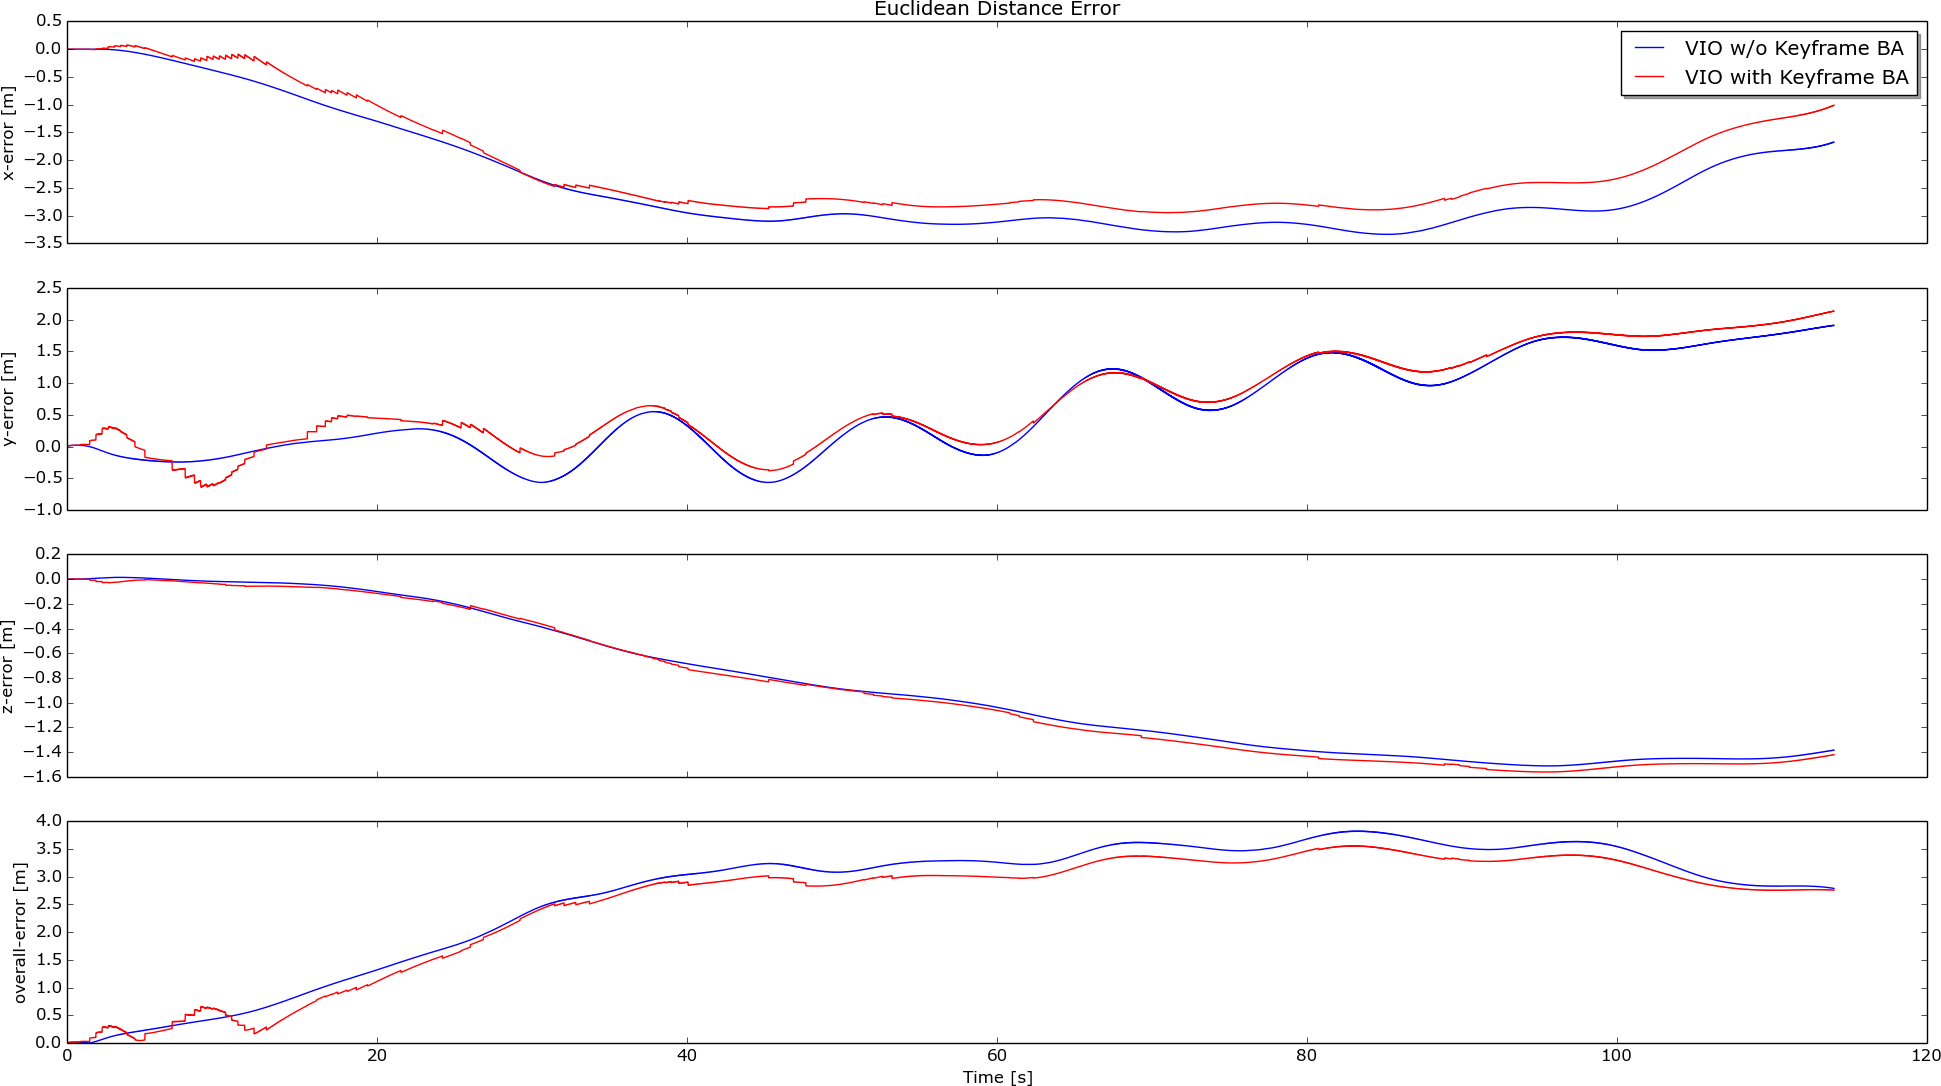
\includegraphics[width=0.45\textwidth]{CONTENT/Figure/figure5_4_a.png}
		\label{fig:fig5-4-a}}
	\end{subfloat}\qquad
	\begin{subfloat}[]{
		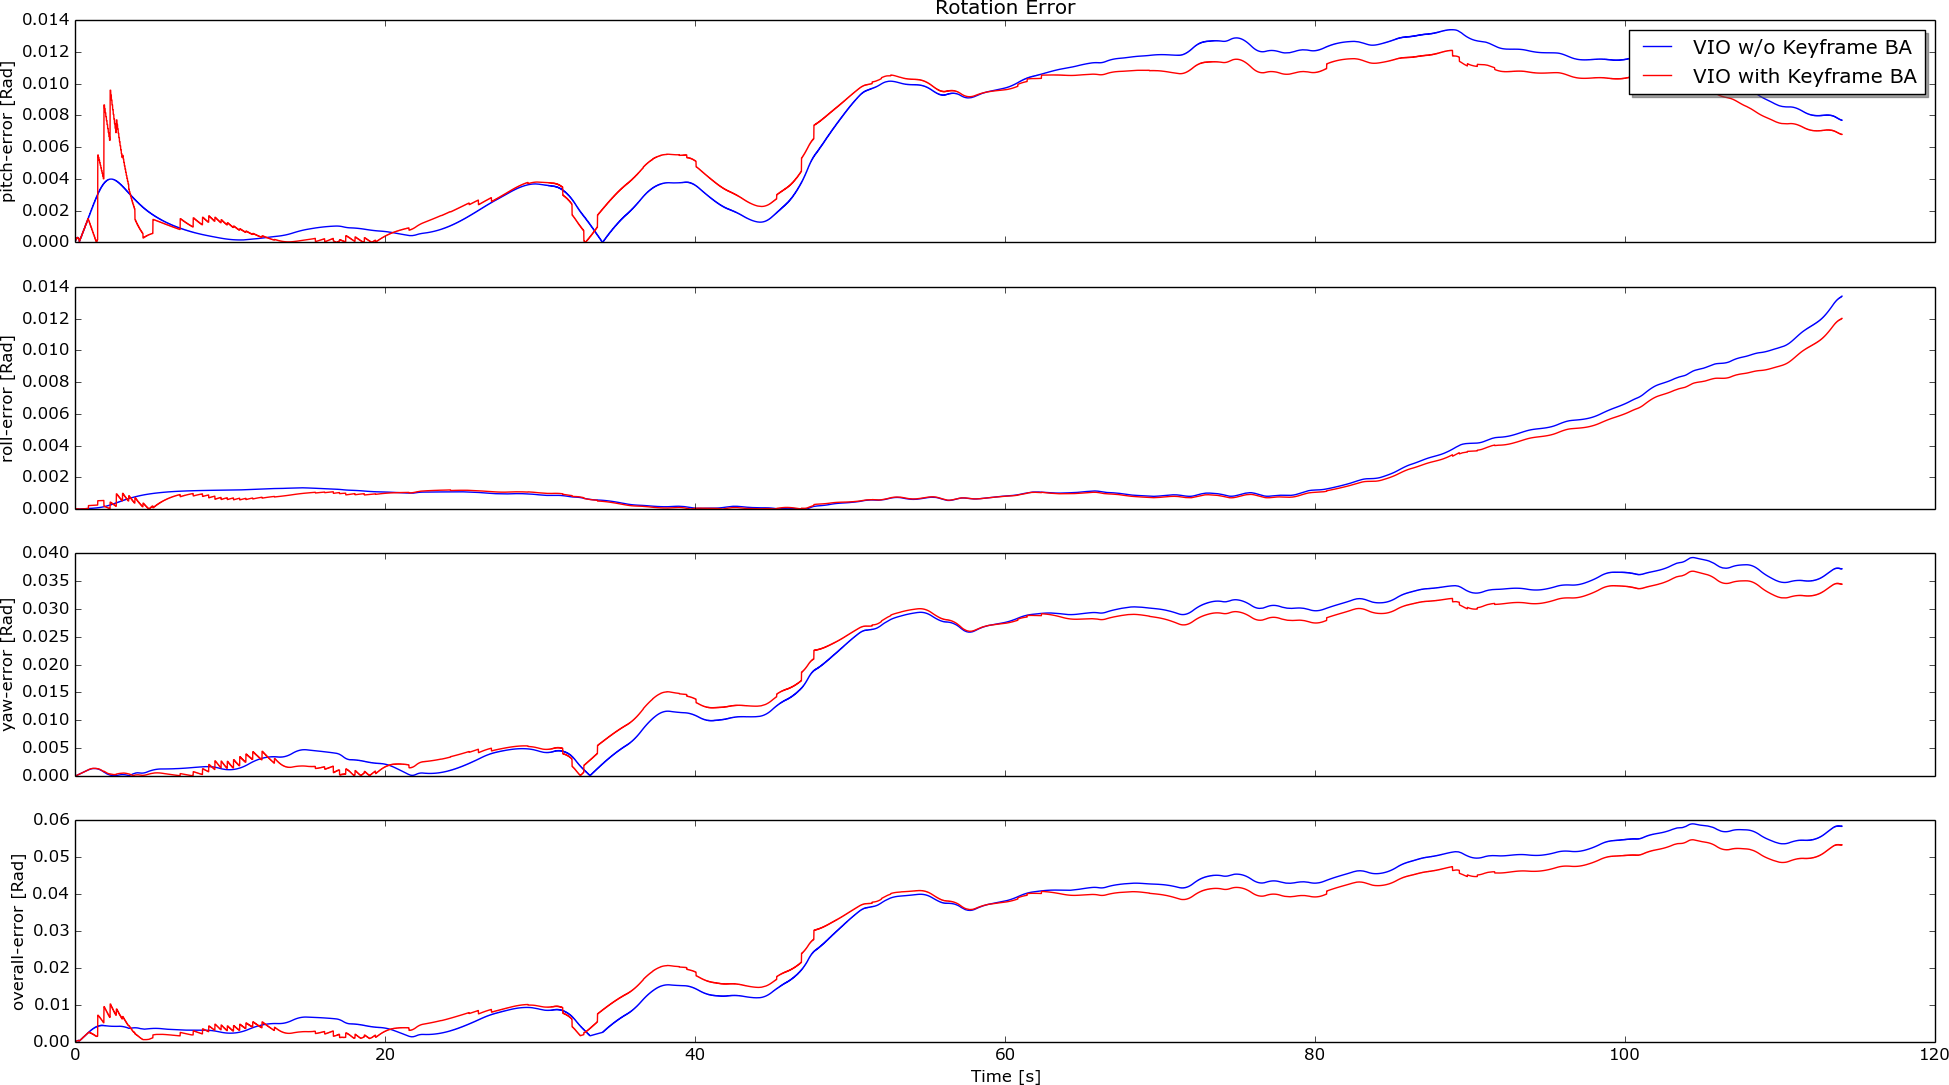
\includegraphics[width=0.45\textwidth]{CONTENT/Figure/figure5_4_b.png}
		\label{fig:fig5-4-b}}
	\end{subfloat}
	
	%\hspace*{\fill} % separation between the subfigures
	
	\caption{Experiment 3: (a) Position drifts of VIO with and without BA. (b) Attitude drifts of VIO with and without BA. The red and blue curves show the errors for VIO with and without keyframe BA respectively.} 
	\label{fig:fig5-4}
\end{figure}

\subsection{Experiment 4: Runtime Evaluation}
\label{subsec:experiment4}


\begin{table}[t]
\centering
\begin{tabular}{|c | P{4cm} |} 
\hline
\ & Time Consuming [ms] \\
\hline
ESKF Prediction & 0.0146\\
Visual Odometry & 4.4656\\
ESKF Correction & 0.0422\\
Keyframe BA & 0.2671\\
\hline
\textbf{Total Visual-Inertial Odometry} & 4.7913\\
\hline

\end{tabular}
     \caption{Experiment 4: Break-up timing results.}
    \label{table:tb5}
\end{table}

\begin{table}[t]
\centering
\begin{tabular}{|c | P{7cm} | P{3cm} | } 
\hline
Name & Parameter Name & Value \\
\hline
\multirow{2}{*}{ESKF IMU} & Nominal state integration & Euler \\
				& Error state integration & Truncated Euler \\
\hline
\multirow{2}{*}{VO} & Max number of features per image & 120 \\
				& Max number of keyframes & 20 \\
\hline
\multirow{2}{*}{Keyframe BA} & Max number of camera poses & 20 \\
				& Max number of iterations & 10 \\
\hline
\end{tabular}
     \caption{Experiment 4: parameter settings in experiment 4. We hereby utilize the similar settings as we explained in experiment 1, 2, and 3.}
    \label{table:tb4}
\end{table}

Table \ref{table:tb5} shows a break-up of average time consumings for single IMU measurement to estimate camera motion in our synthetic datasets. In this experiment, we follow the parameter settings with former experiments, which explicitly shows in Table \ref{table:tb4}. We run experiments on Dataset \textbf{003} and Dataset \textbf{004} 100 times respectively in order to obtain more statistical results.

Though we have shown that our ESKF framework runs in constant time complexity, the whole VIO spends most of time on VO part. For VO part, we use \textit{Fast} parameter settings as \cite{forster2014svo} suggests, except that we compromise the maximum keyframe number to 20 in order to obtain a more accurate pose estimations . The whole system runs smoothly in real-time with our virtual IMU sensor and camera settings, which needs 4.7913 [ms] to process single IMU measurement. 

We conclude that the VIO we suggest in this master thesis have the ability to accomplish a real-time navigation task. It will further be significantly speed-up when more efficient and robust VO has been exploited.

\section{Conclusion}
\label{sec:exp_conclusion}

We first explain the reasons and ways we generate synthetic datasets in this chapter. Then we demonstrate four experiments on our synthetic dataset. In experiment 1, we use the ground truth data in correction step, showing that if the extrasensory data gives us an accurate camera pose estimation, our visual-inertial odometry would have rather small position drift (less than 0.55\% of overall distance travelled) and attitude drift (average 0.0134 [rad]). In experiment 2, we compare our visual-inertial odometry with state-of-art visual odometry \textit{SVO}, the final results show that our method have less variation in position drift and large improvements (0.027 [rad] vs. 0.787 [rad]) in average attitude drift than SVO. In the third experiment, we further show that the keyframe BA we propose decreases the average position drifts and attitude drifts. We examine the break-up time consumptions in experiment 4, that our odometry runs in real-time with our virtual IMU (\~ 100 [Hz]) and camera (\~ 25 [Hz]).

Due to the time limits of this thesis, we are not available to perform more evaluations, \eg, using different visual odometries or applying our system on more realistic datasets. However the results we obtain in above experiments have shown that the keyframe-based visual-inertial odometry we suggest is robust and efficient . 